\documentclass[letterpaper,english, 12pt]{scrreprt}
\usepackage[T1]{fontenc}
\usepackage{array}
\usepackage{graphicx}
\usepackage{float}
\usepackage{titlepic}
\usepackage{multirow}
\usepackage{verbatim}
\usepackage[bookmarks=true]{hyperref}

\newcolumntype{C}[1]{>{\centering\let\newline\\\arraybackslash\hspace{0pt}}m{#1}}

\title{Musical Heart Rate Adjuster}
\author{Group \#12 \\ https://github.com/revan/HeartRateAdjuster \\ 
\\Kenny Bambridge, Jonathan Chang, Samani Gikandi,
\\Tae-Min Kim, Nikhil Shenoy, Revan Sopher}

%\textsc{Software Engineering 14:332:452}

\begin{document}
\titlepic{
\includegraphics{img/title.png}}
\maketitle

\tableofcontents
\newpage

\section{Product Ownership}
Our team will be divided into three smaller sub-teams of two individuals. Each sub-team will be responsible for developing a specific sub-product during the bulk of their time. Upon completion of a significant portion of work, they will provide a brief description of their activity before they push it to our Github repository. In addition to documentation, they will also include the necessary UML diagrams, charts, algorithms, and source code. Every week, or at least once before each deliverable, we will meet together for 1-3 hours during a timeframe determined by a combination of GroupMe and When2meet. During the meeting, we will have a specific agenda that primarily involves the week's progress and upcoming deliverable. Our discussion will probably be centered along the following questions: 1) What did you work on this past week? 2) What do you plan on working on next week? 3) Are there any revisions that need to be made to the project? Every week, a team member will take the lead for the next deliverable to ensure that everything is on time.
corollary
\begin{itemize}
    \item Revan and Tae-Min will work on the general user interface of the mobile application. They will design the layout and basic functionality of the Android app, and set up the communication protocol between the heart rate monitor and the phone. 
    \item Kenny and Samani will work on the music aspect of the mobile application. They will study music playback features such as track selection and queuing to provide customers with a seamless music player experience. They will also be responsible for the nuances of audio playback such as crossfading transitions and tempo adjustments.
    \item Jon and Nikhil will work on the data logging faculties that are necessary to provide the user with feedback about his/her workout. They will work with a server that captures heart rate and music data from the phone and possibly directly from the heart rate monitor. They will determine how to process this information on the server and create customizable graphical displays for user's to view.
\end{itemize}

\begin{comment}
\section{Breakdown of Responsibilities}
\begin{center}
        \begin{tabular}{|C{2cm}|C{6cm}|C{3cm}|C{3cm}|}
                \hline
                         & \textbf{Past} & \textbf{Present} & \textbf{Future}  \\
                \hline
                        \textbf{Jonathan} & Problem Statement, Enumerated Functional Requirements, Preliminary Design, References & Plan of Work & Project Management, Interaction Diagrams, Class Diagrams \\
                \hline
                        \textbf{Kenny} & User Effort Estimation & Domain Analysis & System Architecture and System Design \\
                \hline
                        \textbf{Nikhil} & Enumerated Nonfunctional Requirements, Use Cases (Casual Description, Traceability Matrix, Fully-Dressed Description) & System Operation Contracts & Project Management, Interaction Diagrams, Class Diagrams  \\
                \hline
                        \textbf{Revan} & On-Screen Appearance Requirements, Use Case Diagrams & Mathematical Model & Class Diagrams, System Architecture and System Design \\
                \hline
                        \textbf{Samani} & System Sequence Diagrams & Domain Analysis & System Architecture and System Design \\
                \hline
                        \textbf{Tae-min} & Glossary of Terms, Stakeholders, Actors, Goals & System Operation Contracts & Algorithms and Data Structures \\
                \hline   
                       
        \end{tabular}
\end{center}
\end{comment}
\begin{comment}
\chapter{Interaction Diagrams}
    %These need to be redone
    %\begin{figure}[H]
    \centering
    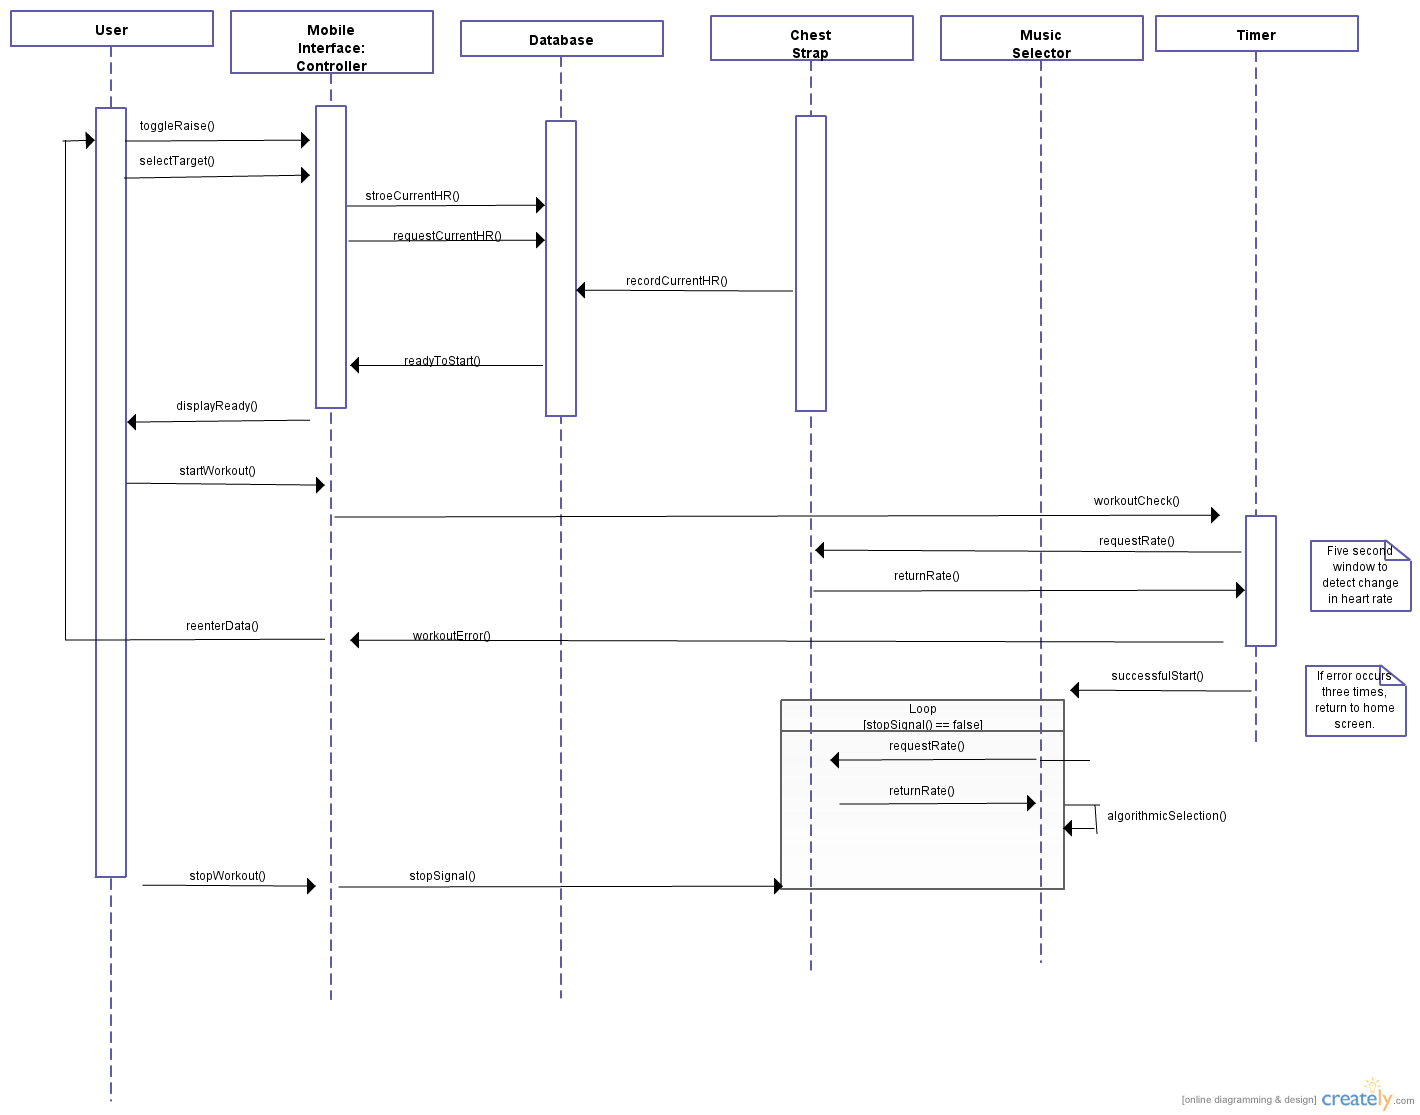
\includegraphics[scale=.35]{img/Interaction_Diagrams/newUC1.png}\\
    \caption {Interaction diagram for the increaseHeartRate case} 
\end{figure}


Since our first two use cases are very similar, we only include the interaction diagram for UC-1, increaseHeartRate. Again, the user toggles the ``raise'' button from the home screen and scrolls to the desired BPM. The database manager coordinates with the heart rate monitor and uses its own algorithm to determine the appropriate song for the music player to play for the user. Then, it waits five seconds for the user to begin his workout. Upon playback, the database manager continuously receives the user's current BPM and makes adjustments to the song's tempo accordingly.

\begin{figure}[H]
    \centering
    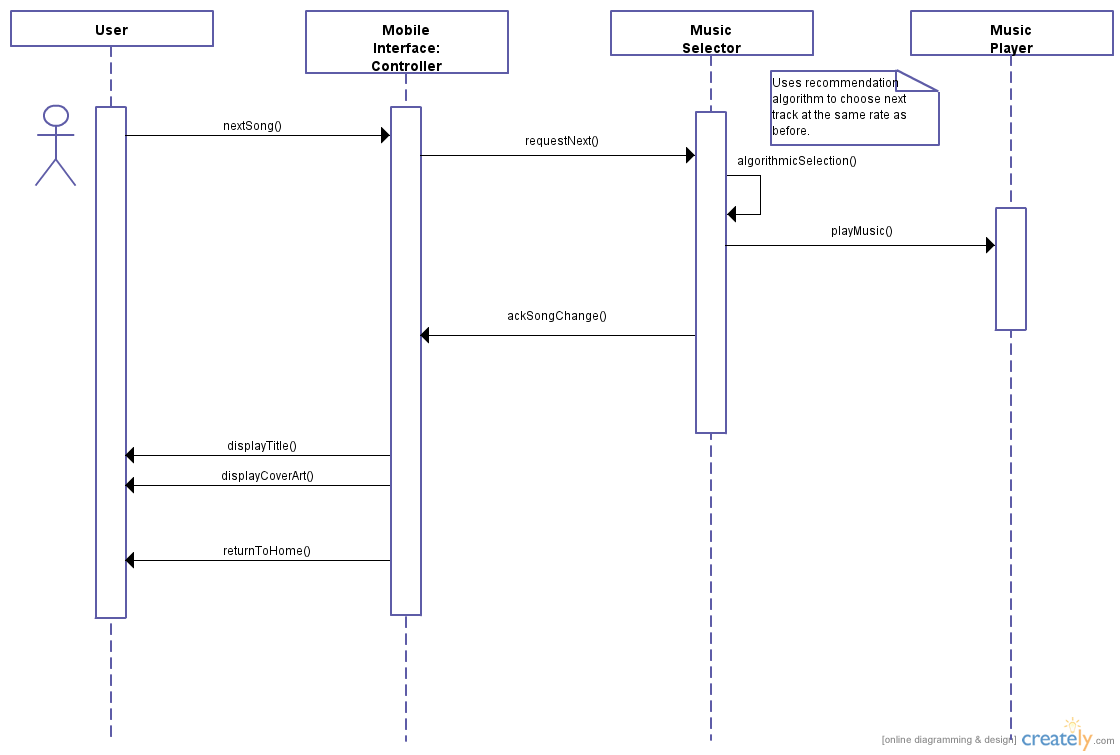
\includegraphics[scale=.40]{img/Interaction_Diagrams/newUC3.png}\\
    \caption {Interaction diagram for getNextSong()} 
\end{figure}

For our third use case, the user's goal is to listen to another song. Similar to the ``skip'' button on most standard music players, we included a double fast-forward arrow for users' convenience. When pressed, the controller immediately contacts the database manager. The database manager selects another track based on its song-selection algorithm for the music player to play. (If the user is currently trying to change his/her heart rate, the database manager will take that into count and select a song of a similar speed.) It also returns the cover art and new song title for the mobile interface to display.

\begin{figure}[H]
    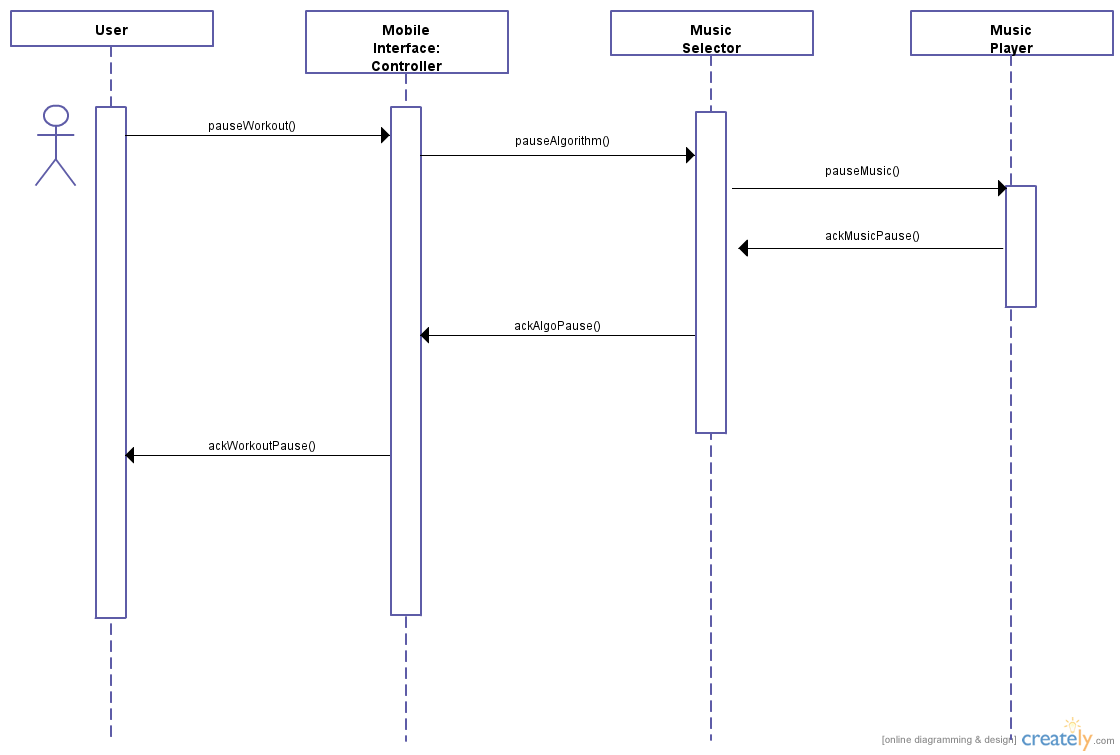
\includegraphics[scale=.40]{img/Interaction_Diagrams/newUC4.png}\\
    \caption {Interaction diagram for pausePlayback()} 
\end{figure}

Our pausePlayback sequence is fairly simple. The user initiates the request by tapping the play/pause button. Then the controller informs the database manager to store the current state settings for future use, and the database manager proceeds to stop recording data and allows the music player to stop the song. The mobile display also updates accordingly.

\begin{figure}[H]
    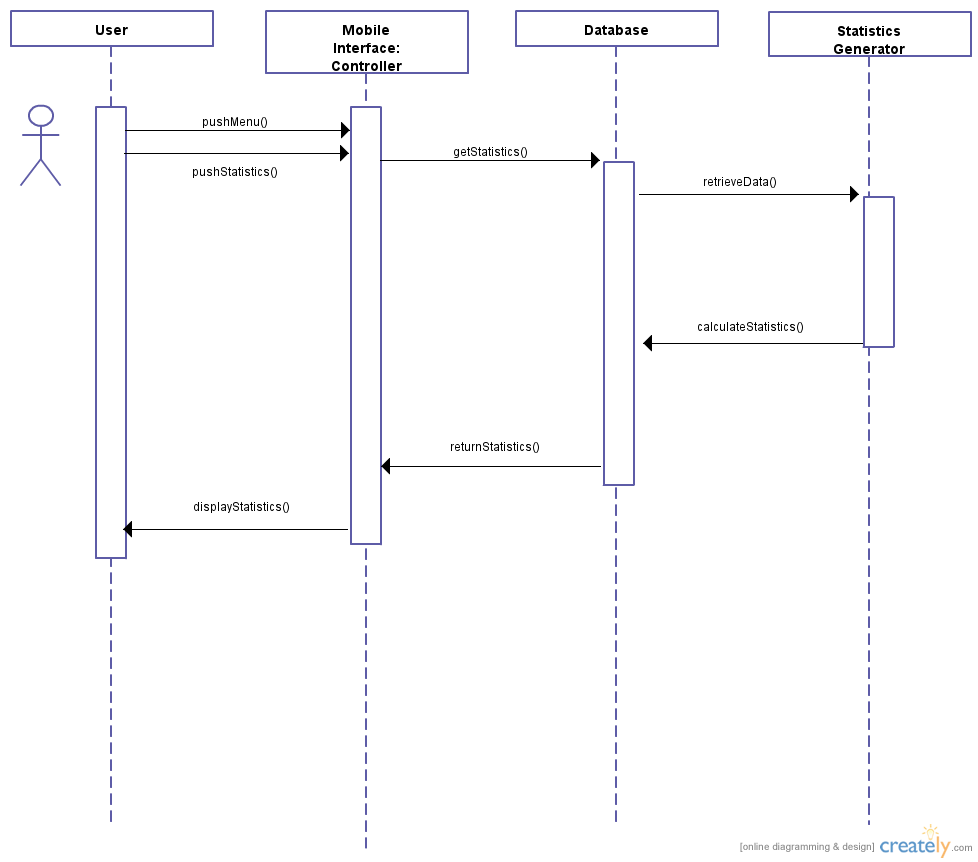
\includegraphics[scale=.40]{img/Interaction_Diagrams/newUC5.png}\\
    \caption {Interaction diagram for getStatistics()} 
\end{figure}
In UC-5, getStatistics, the user begins with two button presses to achieve their goal. First, they bring up the menu button in the top right hand corner and then press ``Statistics'' from the dropdown. The controller passes this request to the database manager, which quickly retrieves and updates the data. Then, it calculates statistics, creates some graphs, and then returns the output to the controller to display. (Note that the user must select from the options available in order to view his workout history.)

\begin{figure}[H]
    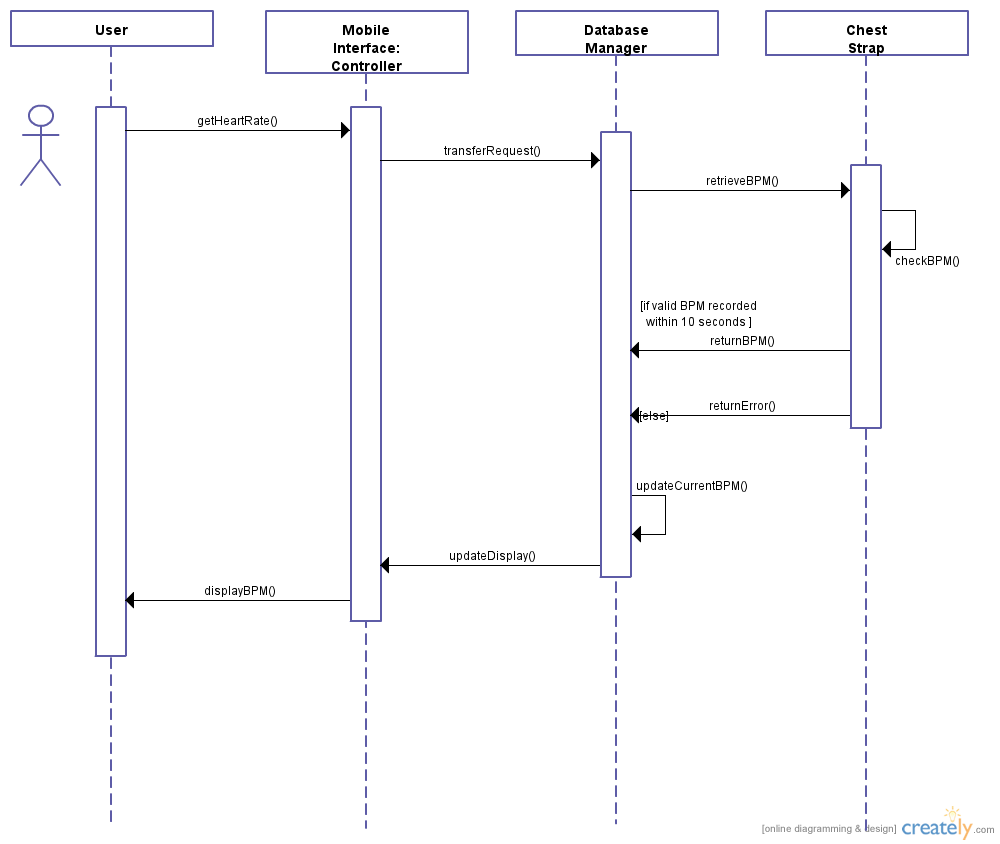
\includegraphics[scale=.40]{img/Interaction_Diagrams/newUC6.png}\\
    \caption {Interaction diagram for getHeartRate()} 
\end{figure}

UC-6, getHeartRate is very similar to UC-5. This use case is also applicable for UC-1, because the Heart Rate is important, needing to be determined continuously. The controller takes the request from the user and passes it to the database manager to handle. The database manager then takes the current BPM value from the Heart Rate Monitor and updates the value for the mobile interface to display to the user. 


\section{Alternate Scenarios}
\begin{figure}[H]
    \centering
    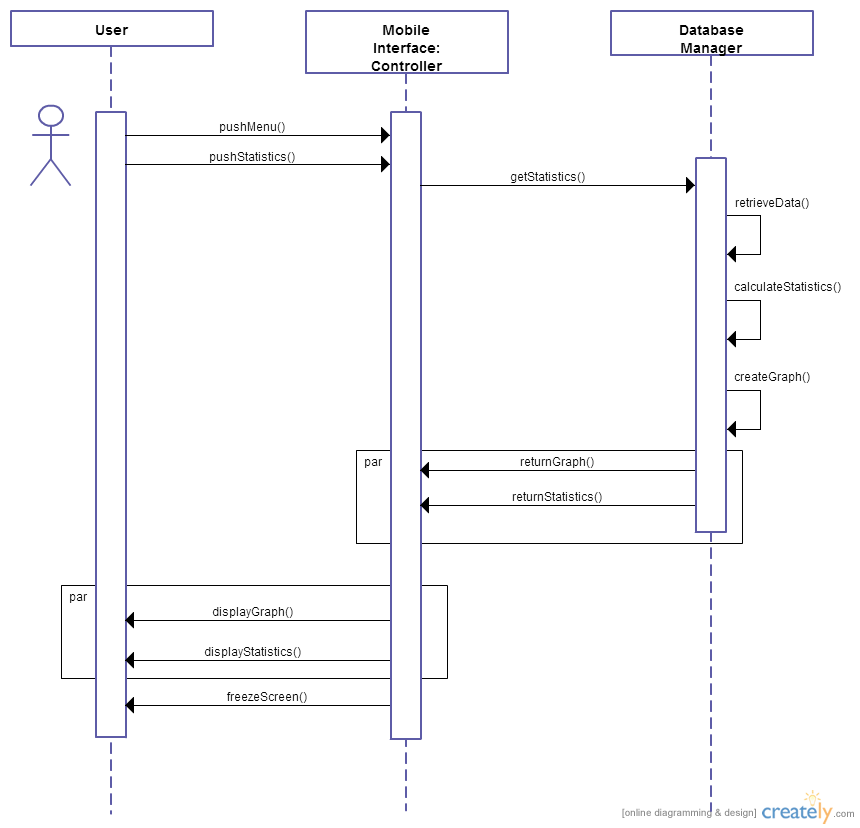
\includegraphics[scale=.30]{img/Interaction_Diagrams/UC-5_getStatistics.png}\\
    \caption {Alternate interaction diagram for getStatistics without the Statistics Generator Object}
    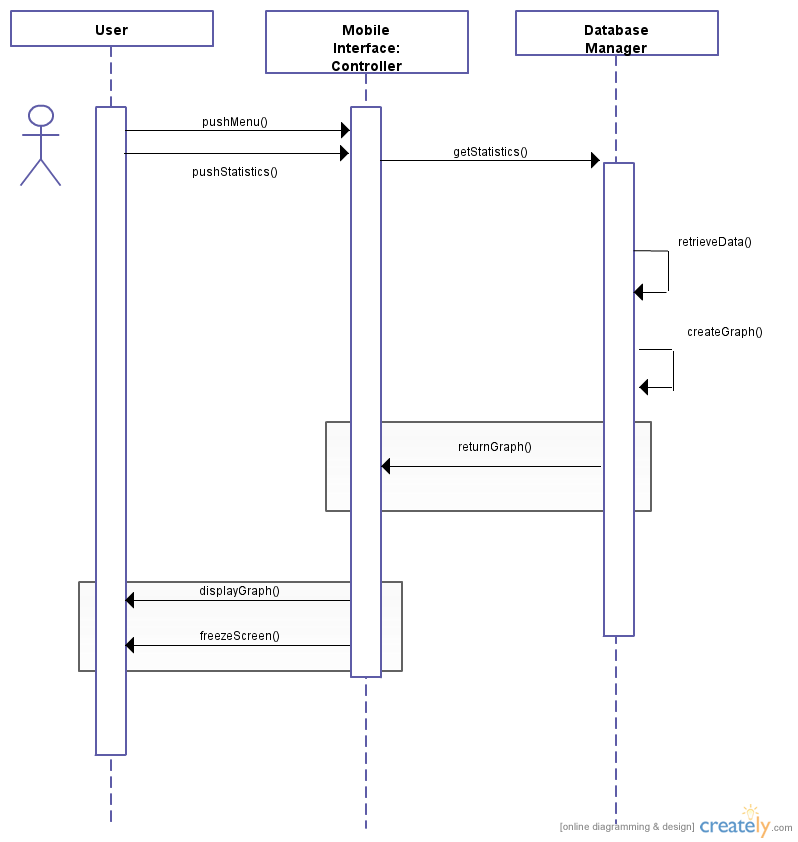
\includegraphics[scale=.30]{img/Interaction_Diagrams/getStatisticsAlternateGraphs.png}\\
    \caption {Alternate interaction diagram for getStatistics() using getGraphs()} 
\end{figure}

\begin{figure}[H]
    \centering
    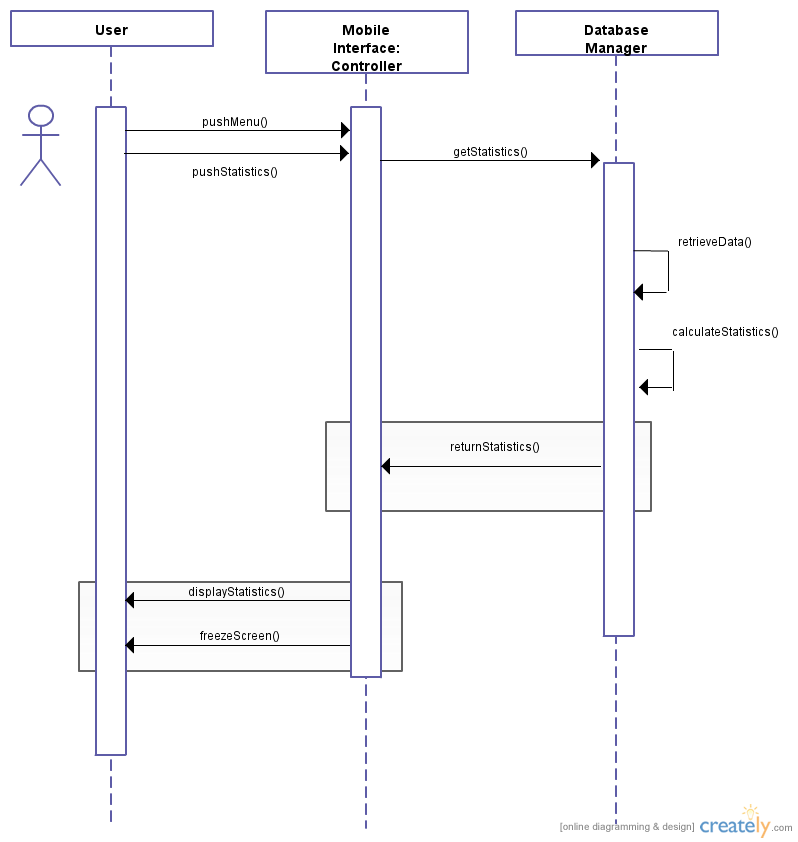
\includegraphics[scale=.30]{img/Interaction_Diagrams/getStatisticsAlternateNumbers.png}\\
    \caption {Alternate interaction diagram for getStatistics() using calculateStatistics()} 
\end{figure}




Alternate scenarios could occur mainly during the getStatistics() use case. Here, the user can select which particular graphs or data he may want to see. In the original diagram, a dedicated Statistics Generator object was created to handle the organization and creation of all statistics. This object greatly simplifies the displayStatistics() case because all the calculations are done outside of the database. However, this is not the only way to solve the case, with the alternative solution being that the statistics are generated directly by the database. Advantages of this are that there is no need to transfer the data between two objects and worry about the communication scheme between them. Also, the time needed to flesh out an entirely new class to handle the calculations would be eliminated. Three different scenarios of keeping the statistics-generation functionality are displayed above. In these diagrams, it is assumed that the user has selected all the options available for getStatistics(), and thus all the graphs and statistics available to the database are displayed to the user. This may not always be the case, as some users may prefer to see graphs only, or numbers only. Some users would like to see a certain combination of both. Thus, our alternate scenarios for the getStatistics() consist of various combinations of all the different display options. For simplicity, only the cases for displaying only graphs and for displaying only numbers are shown in separate interaction diagrams. 

Although keeping the statistics-generation functionality can be contained entirely within the database, we implemented it within a Statistics Generator object. This decision was made to keep consistency with the High Cohesion and Low Coupling Principles. If we hadn`t made the separation, then the database would have too many responsibilities to take care of. By creating a dedicated Statistics Generator object, the statistics can be fully fleshed out and managed without having to worry about other responsibilities.

\section{Design Patterns}

This project was developed through a mainly object-oriented approach. We were able to boil our system down to a few, distinct actors, and an object-oriented approach seemed appropriate to model our system. As evidenced by the interaction diagrams, there are five main actors: the user, the mobile interface, the database, the music player, and the heart rate monitor. Each of these actors has a specific set of actions that they can perform, and these actions are not very tightly coupled to those of other actions in the system. For example, the music player is designated to solely play the music on the device. It does not have access to the music algorithm or the heart rate; its sole job is to respond to requests about playing or pausing the music. Similarly, the database manager is solely responsible for manipulating data and handling requests. These characteristics are prime examples of the High Cohesion principles, because each actor in the system has its own specific tasks, and the respective actors are designed to that their tasks are carried out very well. We acknowledge that some of the actors are more important than the others, such as the database manager and the mobile interface, but this is out of necessity. The user interacts directly with the interface, and the interface talks directly to the database in most cases. The other objects in the system are more supplementary in the sense that they carry out the commands given to them by the database-mobile-interface pair. Although there is some communication between the different objects, the communication has been designed such that each method call is specific, efficient, and effective. This cuts back on unnecessary communication between the objects and allows for the system to be optimized. The Low Coupling Principle requires that objects should ``not take on too many communication responsibilities'', and our design fulfills the requirement because we have minimized the number of interactions to just the necessary ones. All in all, our object-oriented design encompasses aspects from both the High Cohesion and Low Coupling principles, and creates and effective solution to the heart rate monitoring problem.

\section{Assignment of Responsibilities}

A prime example can be found in UC-4, pausePlayback. Each object submits a request to the next object in line before reaching the Music Player, which is supposed to fulfill the ``pause'' function. At this point, the interactions start coming back. It is clearly seen that each object in this example transmits at most two messages, and no object performs more than a single computation. A similar theme exists in UC-6, getHeartRate. Each object essentially sends one message and receives one message. Furthermore, each object does not need to fulfill more than two active responsibilities. We believed that by distributing the workload for each object through the High Cohesion Principle and the Low Coupling Principle, we would be reaching the best balance.
The Expert Doer Principle was not followed as closely because the communication links of the objects we used are a bit longer. In our design, the ``one who knows'' often passes on the knowledge to another object that ``needs to know'' before the task is actually fulfilled. For instance, the Database Manager often causes the Controller to update the display and show the user rather than directly communicating with the user. Basically, our Controller and Database Manager are both extremely important, so oftentimes, they both end up with most of the implementation details.
\end{comment}
\chapter{Class Diagrams and Interface Specification}

\section{Class Diagrams}
    \subsection{Audio BlackBox Subsystem}
    \begin{center}
    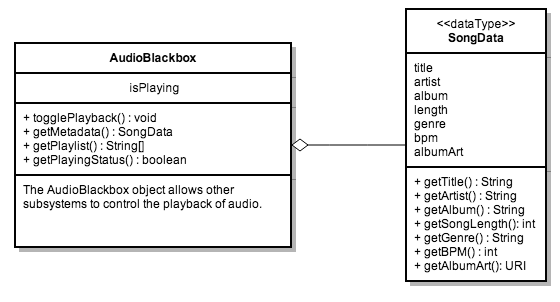
\includegraphics[width=.9\textwidth]{img/ab/class_diagrams/audioblackbox_cd.png} \\
\end{center}

\subsection{General UI \& Hardware Subsystem}
    \begin{center}
    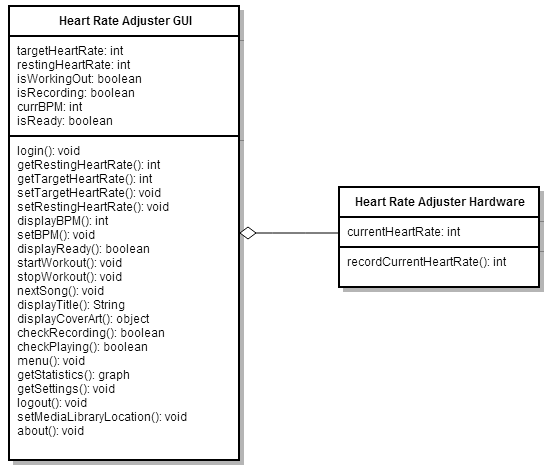
\includegraphics[width=.9\textwidth]{img/ui/HartRateAdjusterGUI_UML.png} \\
\end{center}
 
\subsection{Data Logging and Display Subsystem}
    \begin{center}
    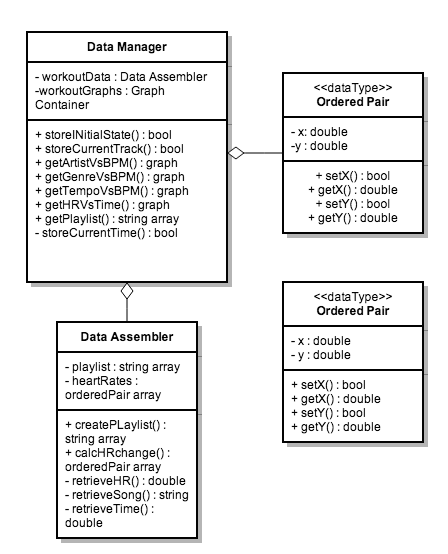
\includegraphics[width=.9\textwidth]{img/dm/Class_Diagrams/datamanagement_cd.png}
\end{center}



\section{Data Types and Operation Signatures}
    \subsection{Audio BlackBox Subsystem}
    %\input{2.2.b+ab}
\subsection{General UI \& Hardware Subsystem}
    %\begin{center}
	\begin{tabular}{|C{15cm}|}
		\hline
			\textbf{Heart Rate Adjuster GUI} \\
		\hline
			\begin{flushleft}
				\textbf{Variables:} \\
			\end{flushleft}
				\begin{itemize}
					\item targetHeartRate: int. This variable will store the target heart rate for the user's workout. This variable is private but can be accessed and changed from other methods.
					\item restingHeartRate: int. This variable will store the user's initial resting heart rate before the workout begins. This variable is private but can be accessed and changed from other methods.
					\item isWorkingOut: boolean. This variable will store data on whether the application detects that the user is currently working out or not.
					\item isRecording: boolean. This variable will store data on whether the application is recording the user's heart rate or not.
					\item currBPM: int. This variable will store the BPM of the current track that is playing.
					\item isReady: boolean. This variable will store data on whether the system is ready to begin or not.
				\end{itemize} \\
			\hline
			\begin{flushleft}
				\textbf{Functions: } \\
			\end{flushleft}
				\begin{itemize}
					\item login(): void. This function will log the user in to a new session, keeping session persistence.
					\item getRestingHeartRate(): int. This function will return the data stored in variable targetHeartRate.
					\item getTargetHeartrate(): int. This function will return the data stored in variable currentHeartRate.
					\item setTargetHeartRate(): void. This function will set the data stored in variable targetHeartRate to equal the given parameter.
					\item setRestingHeartRate(): void. This function will set the data stored in variable restingHeartRate to equal the given parameter.
					\item displayBPM(): int. This function will return the data stored in variable currBPM.
					\item setBPM(): void. This function will set the data stored in variable currBPM to the passed parameter.
					\item displayReady(): boolean. This function will return the data stored in variable isReady.
					\item startWorkout(): void. This function will initiate the workout and attempt to adjust the currentHeartRate toward the targetHeartRate.
					\item stopWorkout(): void. This function will stop the workout from continuing its functions.
					\item nextSong(): void. This function will skip the current track which is being played, and use the algorithm to play the next appropriate song.
					\item displayTitle(): String. This function will display the title of the currently playing track.
					\item displayCoverArt(): object. This function will display the cover art of the currently playing track.
					\item checkRecording(): boolean. This function will return the data stored in the variable isReady.
					\item checkPlaying(): boolean. This function will return the data stored in the variable isREady.
					\item menu(): void. This function will display the menu for the application.
					\item getStatistics(): graph. This function will return graphs which contain statistics from the data manager.
					\item getSettings(): void. This function will display the settings for the application.
					\item logout(): This function will log the current user out of their current session.
					\item setMediaLibraryLocation(): void. This function will set the library location of the media which is to be  used for the application.
					\item about(): This function will display the "about" information for the application.
				\end{itemize}
			\hline
	\end{tabular}
\end{center}

\begin{center}
	\begin{tabular}{|C{15cm}|}
		\hline
			\textbf{Heart Rate Adjuster Hardware} \\
		\hline
			\begin{flushleft}
				\textbf{Variables:} \\
			\end{flushleft}
				\begin{itemize}
					\item currentHeartRate: int. This variable will store data on the user's current heart rate, as measured by the hardware device.
				\end{itemize} \\
			\hline
			\begin{flushleft}
				\textbf{Functions: } \\
			\end{flushleft}
				\begin{itemize}
					\item recordCurrentHeartRate(): int. This function will retrieve the current heart rate of the user as measured by the hardware device and update the variable currentHeartRate.
				\end{itemize}
			\hline
	\end{tabular}
\end{center}
\subsection{Data Logging and Display Subsystem} 
    \begin{center}
    \begin{tabular}{|C{15cm}|}
        \hline
            \textbf{Data Manager}\\
        \hline
            \begin{flushleft}
                \textbf{Variables:} \\
            \end{flushleft}
                \begin{itemize}
                    \item workoutData: Data Assembler. This is a Data Assembler object which stores the data points retrieved from storage. It also stores the songs and their metadata.
                    \item workoutGraphs : Graph Container. This is a Graph Container object which stores the different graphs that were requested by the User Interface.
                \end{itemize} \\
            \hline
            \begin{flushleft}
                \textbf{Functions:} \\
            \end{flushleft}
                \begin{itemize}
                    \item storeInitialState(double initialRate, double targetRate) : bool. This function stores the initial state of the system, which is captured in the form of the user's initial heart rate and the target heart rate.
                    \item storeCurrentTrack(string song) : bool. This function is used by the Music Module to store the current track being played. This information is later used for the playlist.
                    \item storeCurrentHR(double heartRate) : bool. This function is used to store the current heart rate into the data storage. It is used by the User Interface while the user is working out with the system.
                    \item getArtistVsBPM() : graph. This function will access the data stored in the Data Assembler and create a histogram displaying the artist who's songs were played most often at different BPMs. The Data Manager will select the appropriate graph from the Graph Container and return it to the UI.
                    \item getGenreVsBPM() : graph. This function will create a histogram of the most frequent genres at different BPMs. The data will be accessed from the Data Assembler and plotted by the Graph Container. The final graph will be selected by the Data Manager from the Graph Container
                    \item getTempoVsBPM() : graph. This function will return a graph of the music's tempo versus the user's BPM.
                    \item getHRvsTime() : graph. This function will return a graph of the user's heart rate over time.
                    \item getPlaylist(): string array. This function will return an array of the music that was played during the workout.
                    \item storeCurrentTime() : bool. This is an auxiliary function which stores the current system time in the data storage every time storeCurrentHR() is called. It will associate the time with the current heart rate.
                \end{itemize}
                \\
            \hline
    \end{tabular}
\end{center}

\begin{center}
    \begin{tabular}{|C{15cm}|}
        \hline
            \textbf{Data Assembler} \\
        \hline
            \begin{flushleft}
                \textbf{Variables:} \\
            \end{flushleft}
                \begin{itemize}
                    \item playlist: string array. This variable will store the names of the songs that were played during the workout.
                    \item heartRates: Ordered Pair array. This variable will store the retrieved data points in ascending order.
                \end{itemize} \\
            \hline
            \begin{flushleft}
                \textbf{Functions: } \\
            \end{flushleft}
                \begin{itemize}
                    \item createPlaylist() : string array. This function will fetch the songs played during the workout from the data storage and arrange them in the playlist array and return it.
                    \item calcHRchange() : orderedPair. This function will retrieve all the heart rates and system times from the data storage and organize them into ordered pairs. The ordered pairs are stored in an array and returned to the caller.
                    \item retrieveHR() : double. This function retrieves a heart rate from the data storage.
                    \item retrieveTime() : double. This function retrieves a time from the data storage.
                    \item retrieveSong() : string. This function retrieves a song name from data storage.
                \end{itemize}
                \\
            \hline
    \end{tabular}
\end{center}

\begin{center}
    \begin{tabular}{|C{15cm}|}
        \hline
            \textbf{Graph Container} \\
        \hline
            \begin{flushleft}
                \textbf{Variables:} \\
            \end{flushleft}
                \begin{itemize}
                    \item graphs : graph array. This variable contains an array of the different graphs that were requested by the User Interface.
                \end{itemize} \\
            \hline
            \begin{flushleft}
                \textbf{Functions: } \\
            \end{flushleft}
                \begin{itemize}
                    \item createArtistVsBPM(Data Assembler workoutData) : bool. This function takes the names of the artists and heart rates stored in the Data Assembler and graphs them against each other.
                    \item createGenreVsBPM(Data Assembler workoutData) : bool. This function graphs the genre of the music versus the user's heart rate using the data from workoutData.
                    \item createTempoVsBPM(Data Assembler workoutData) : bool. This function graphs the tempo of the music versus the user's heart rate using the workoutData object.
                    \item createHRVsTime(Data Assembler workoutData) : bool. This function graphs the user's heart rate versus time using the workoutData object.
                \end{itemize}
                \\
            \hline
    \end{tabular}
\end{center}

\begin{center}
    \begin{tabular}{|C{15cm}|}
        \hline
            \textbf{Ordered Pair} \\
        \hline
            \begin{flushleft}
                \textbf{Variables: }\\
            \end{flushleft}
                \begin{itemize}
                    \item x : double. This variable stores the x-coordinate of the data point.
                    \item y : double. This variable stores the y-coordinate of the data point.
                \end{itemize} \\
            \hline
            \begin{flushleft}
                \textbf{Functions: } \\
            \end{flushleft}
                \begin{itemize}
                    \item setX(double newX) : bool. This function sets the value of the variable x.
                    \item getX() : double. This function returns the current value of the variable x.
                    \item setY(double newY) : bool. This function sets the value of the variable y.
                    \item getY() : double. This function returns the current value of the variable y.
                \end{itemize}
                \\
            \hline
    \end{tabular}
\end{center}


\section{Traceability Matrix}
    \subsection{Audio BlackBox Subsystem}
    \begin{center}
    \begin{tabular}{|l|c|}
        \hline
        \textit{Domain Concepts}    &   \textbf{AudioBlackbox}
        \\ \hline

\textbf{HRM Manager}        &       \\ \hline
\textbf{Log Retriever}      &       \\ \hline
\textbf{Track Logger}       &       \\ \hline
\textbf{Music Playerbacker} &   X   \\ \hline
\textbf{Track Queuer}       &   X   \\ \hline
\textbf{General UI}         &   X   \\ \hline
\textbf{Playback View}      &   X   \\ \hline
\textbf{Heart Beat View}    &       \\ \hline
\textbf{Workout View}       &       \\ \hline
\textbf{History View}       &       \\ \hline
\textbf{Workout Store}      &       \\ \hline
\textbf{Metadata Store}     &   X   \\ \hline
\textbf{Music Store}        &   X   \\ \hline

    \end{tabular}
\end{center}

\subsection{General UI \& Hardware Subsystem}
    %\begin{center}
 	\begin{tabular}{|l|C{3cm}|C{2.5cm}|C{2.5cm}|C{2.5cm}|C{2.5cm}|}
 		\hline
 			&  \multicolumn{4}{|c|}{\textit{Class}} \\  \hline
 
 			\textit{Domain Concepts}	&	\textbf{Data Manager}	&	\textbf{Data Assembler}	&	\textbf{Graph Container}	& \textbf{Ordered Pair} & \textbf{Heart Rate Monitor GUI} & \textbf{Heart Rate Monitor Hardware}	\\ \hline
 
 \textbf{HRM Manager}		&	X	&		&		&		&		&	X	\\ \hline
 \textbf{Log Retriever}		&	X	&		&		&		&		&		\\ \hline
 \textbf{Track Logger}		&	X	&		&		&		&		&		\\ \hline
 \textbf{Music Playerbacker}	&	X	&		&		&		&	X	&		\\ \hline
 \textbf{Track Queuer}		&	X	&	X	&		&		&		&		\\ \hline
 \textbf{General UI}			&	X	&	X	&		&		&	X	&		\\ \hline
 \textbf{Playback View}		&	X	&	X	&	X	&		&	X	&		\\ \hline
 \textbf{Heart Beat View}		&	X	&	X	&	X	&		&	X	&		\\ \hline
 \textbf{Workout View}		&	X	&	X	&	X	&		&	X	&		\\ \hline
 \textbf{History View}		&	X	&	X	&	X	&		&	X	&		\\ \hline
 \textbf{Workout Store}		&	X	&	X	&		&	X	&		&	\\ \hline
 \textbf{Metadata Store}		&	X	&	X	&		&	X	&		&	\\ \hline
 \textbf{Music Store}		&	X	&	X	&		&	X	&		&	\\ \hline
 
 	\end{tabular}
\end{center}
 
 	From our domain concepts, we derived four classes: data manager, data assembler, graph container, and ordered pair. Our data manager is essentially involved with every domain. Its purpose is to log and manage various types of data, and store the packaged data other objects to retrieve. Essentially, the data manger acts as an intermediary in most steps, but only providing a minimal interface for modules so that data cannot be tampered with or seen, just used.
 
 	Next, our data assembler is charged with retrieving the appropriate data from the database and packaging it in a convenient form for usage. For instance, we can take songs and metadata from their storage locations and return playlists. We can also take our data and create ordered pairs for our graph container. Then, our graph container contains an array of the requested graphs, and it is involved with the domain concepts that require various views. Using our data assembler allows us to have a nice container of data to graph. Finally, our ordered pair class was derived from the storage concepts. We use it to store data points, so that we will be able to access them.

	For the user interface and hardware communication, two other classes were derived rather clearly: the Graphical User Interface class, and the Hardware communication class. The graphical user interface is involved with many domains, save the few domains relating to data storage - that is taken care of by the data manager portion. The purpose of the graphical user interface is for users to be able to easily interact with the application. This includes being able to easily view different portions of the application such as information on their current workout, their history, etc. The next class, Hardware, was derived as a modularized way to communicate with the Heart Rate Monitor which is required to retrieve information about the user's heart rate. This class is simple - it's only function is to receive information from the HRM being used, and to update the user's current heart rate in real time.
\subsection{Data Logging and Display Subsystem}
    \begin{center}
    \begin{tabular}{|l|C{3cm}|C{2.5cm}|C{2.5cm}|C{2.5cm}|C{2.5cm}|}
        \hline
            &  \multicolumn{4}{|c|}{\textit{Class}} \\  \hline
            \textit{Domain Concepts}    &   \textbf{Data Manager}   &   \textbf{Data Assembler} &   \textbf{Graph Container}    & \textbf{Ordered Pair} \\ \hline

\textbf{HRM Manager}        &   X   &       &       &       \\ \hline
\textbf{Log Retriever}      &   X   &       &       &       \\ \hline
\textbf{Track Logger}       &   X   &       &       &       \\ \hline
\textbf{Music Playerbacker} &   X   &       &       &       \\ \hline
\textbf{Track Queuer}       &   X   &   X   &       &       \\ \hline
\textbf{General UI}         &   X   &   X   &       &       \\ \hline
\textbf{Playback View}      &   X   &   X   &   X   &       \\ \hline
\textbf{Heart Beat View}    &   X   &   X   &   X   &       \\ \hline
\textbf{Workout View}       &   X   &   X   &   X   &       \\ \hline
\textbf{History View}       &   X   &   X   &   X   &       \\ \hline
\textbf{Workout Store}      &   X   &   X   &       &   X   \\ \hline
\textbf{Metadata Store}     &   X   &   X   &       &   X   \\ \hline
\textbf{Music Store}        &   X   &   X   &       &   X   \\ \hline

    \end{tabular}
\end{center}

    From our domain concepts, we derived four classes: data manager, data assembler, graph container, and ordered pair. Our data manager is essentially involved with every domain. Its purpose is to log and manage various types of data, and store the packaged data other objects to retrieve. Essentially, the data manger acts as an intermediary in most steps, but only providing a minimal interface for modules so that data cannot be tampered with or seen, just used. \\

    Next, our data assembler is charged with retrieving the appropriate data from the database and packaging it in a convenient form for usage. For instance, we can take songs and metadata from their storage locations and return playlists. We can also take our data and create ordered pairs for our graph container. Then, our graph container contains an array of the requested graphs, and it is involved with the domain concepts that require various views. Using our data assembler allows us to have a nice container of data to graph. Finally, our ordered pair class was derived from the storage concepts. We use it to store data points, so that we will be able to access them.



\chapter{System Architecture and System Design}

\section{Architectural Styles}
    \subsection{Audio BlackBox Subsystem}
    The Audio BlackBox Subsystem uses a Client-Server architecture internally. The server stores and coordinates all audio files/streams as well as the playlist determination logic. The client, in this case a mobile device, abstracts the server's behavior into an interface for retrieving metadata and altering playback. Additionally, the client interfaces with the mobile device's faculties for outputting audio.
\subsection{Data Logging and Display Subsystem}
        Our system utilizes a three-tier architecture system and consists of 3 layers. These include a presentation tier, an application tier, and a data tier. Our presentation layer is primarily represented by our mobile interface which is used to display our application’s relevant information. It also allows the user to interact with our system by inputting commands and accepting outputs. Meanwhile, our application layer consists of logical operations and data access. For example, our song-selection algorithm would be included in this layer. This application layer uses logical operations to convert raw user data into readable results. Finally, our data tier consists of our database where our information is stored and retrieved. \\

    These three tiers are separated from each other to allow for encapsulation and data abstraction. We want each tier to hide its usage from implementation and to preserve the integrity of our data. We also want to reduce the overall complexity of our system. However, each tier must maintain a sufficient level of communication and be able to retrieve needed data from each other. In a common scenario for our system, our application layer may request information from the data tier. It then processes this information and returns it to the presentation tier in response to the user request. A visual diagram was provided in our earlier stage of planning in the section titled System Architecture Diagram.

    
\section{Identifying Subsystems}
        Our software is designed around three primary subsystems. The core subsystem is the UI Subsystem. This subsystem is responsible for interfacing with the user, the chest strap, and provisioning other hardware and software faculties. The Audio BlackBox subsystem handles all audio playback faculties. The Data Logging Subsystem is used for recording data about workouts. Additionally, this subsystem provides faculties for displaying and manipulating logged data. Within each of these subsystems are further subsystems.
    
\subsection{Audio BlackBox Subsystem}
    The Audio Black Box refers to two things. 'AudioBlackbox' is a Java interface that lives on the smartphone. This interface is used by other subsystems of the heartBPM application to control audio playback and get information about the music that's currently playing. In general terms, the Audio Black Box is the entire audio subsystem. It handles the queueing of songs, interfacing with native Android subsystems for playing actual audio streams, and with a server backend.

\section{Mapping Subsystems to Hardware}
    TODO: Samani and Kenny

    
\section{Persistent Data Storage}
    \subsection{Data Logging and Display Subsystem}
        Since Android provides full support for SQLite databases, it is the type of storage that we have chosen for the application. The wide variety of fully-developed features allows us to focus more on the actual organization and management of the data in relation to the other modules. All that is needed is a simple call to the data base to retrieve the raw data, and the custom designed objects illustrated in the Class Diagram then do their own processing on the data. SQLite allows us to store all the data specific to application on the device itself, which is advantageous for a mobile application such as ours. The goal is for the user to be able to record and view his workout data without having to use any external devices other than his phone and the chest strap, and internal data storage via the SQLite database allows our application this benefit. \\
        The database will be accessible only to the Data Manager and the Data Assembler. In regards to the Data Manager, the only interactions with the database will be to store the initial state of the system, store the current music track, and store the current heart rate. It will not retrieve anything from the database, because that is the purpose of the Data Assembler. The Data Assembler is the other object that will interact with the database. It will issue requests for the various data that the UI would like to graph, which include the heart rate, the current times, and the songs. Thus, the Data Manager and Data Assembler are the only objects that have direct access to the database.


\section{Network Protocol}
    \subsection{Audio BlackBox Subsystem}
    The Audio BlackBox uses live streaming and transcoding techniques to provide audio based on media files living on a server. The Transport layer protocol used will likely be TCP. The Application layer will likely use HTTP.
    
\section{Global Control Flow}
    \subsubsection{Execution Orderness}
    Internally, data transfer between the Audio BlackBox server and mobile device is procedural while events can trigger a change in behavior in the way the server behaves.
\subsubsection{Execution Orderness}
The execution order is a mix of procedure-driven and event-driven. From a broad view, the use of the program follows the same steps: the user starts the music, the system runs, then the user stops the music. However, the system provides a variety of interface options to activate events during the execution: a user may pause or skip playback, and view their statistics, at any time.

\subsubsection{Time Dependency}
The system is real-time, with a timer firing once a second.
This timer triggers the fetching of the heart rate from the monitor, and triggers the logging of this data.

\subsubsection{Concurrency}
The Android standard concurrency model is that the main thread handles UI, so lengthy tasks must be performed on a background thread else the UI becomes unresponsive.
As such, the network IO of the music selection system must certainly be in a different thread.
Synchronization is unnecessary as there is no shared resource.




\section{Hardware Requirements}
    The Audio BlackBox Server component requires a server with the processing capacity to transcode media content as well as generate playlists based on the user's activity.
The system requires:
\begin{itemize}
  \item Touch screen display with minimum resolution of 640 x 480 pixels
  \item Storage space for music library, minimum size of 100 Mb
  \item Bluetooth for communication with a heart rate monitor
  \item Network connection for communicating with music selection service
  \item Audio playback capabilities
\end{itemize}
All of these requirements are met by most Android phones on the market.

    


\chapter*{Individual Contributions Breakdown}
\begin{center}
    \begin{tabular}{|l|C{2cm}|C{1.5cm}|C{1.5cm}|C{1.5cm}|C{1.5cm}|C{1.5cm}|}
        \hline
            &   Kenny Bambridge     &   Jonathan Chang      &   Samani Gikandi      &   Tae-Min Kim &     Nikhil Shenoy     &   Revan Sopher\\ \hline
Problem Statement   &       X       &       X       &       X       &       X   &       X       &   X       \\ \hline
Glossary of Terms   &               &               &               &       X   &               &           \\ \hline
System Requirements &               &       X       &               &           &       X       &   X   \\ \hline
Func. Requirements  &               &       X       &               &       X   &               &       \\ \hline
Non-Func. Req.      &               &               &               &           &       X       &       \\ \hline
Appearance Req.     &               &       X       &               &           &               &       X\\ \hline
Stakeholders        &               &               &               &       X   &               &        \\ \hline
Actors and Goals    &               &               &               &       X   &               &        \\ \hline
System Sequence Diagram &               &               &       X       &           &               &        \\ \hline
Preliminary Design  &               &       X       &               &           &               &   X    \\ \hline
User Effort Estimation  &       X       &               &               &           &               &        \\ \hline
Use Cases       &               &               &               &       X   &       X       &   X    \\ \hline
System Sequence Diagrams&               &               &       X       &           &               &        \\ \hline
User Effort Estimation  &       X       &               &               &           &               &        \\ \hline
Domain Model        &       X       &               &       X       &           &               &        \\ \hline
Operation Contracts &               &               &               &       X   &       X       &        \\ \hline
Mathematical Model  &               &               &               &           &               &   X    \\ \hline
Plan of Work        &               &       X       &               &           &               &        \\ \hline
Interaction Diagrams    &               &       X       &               &           &       X       &        \\ \hline
Project Management  &       X       &       X       &       X       &       X   &       X       &       X\\ \hline
LaTeX Maintenance   &       X       &       X       &       X       &       X   &       X       &       X\\ \hline
    \end{tabular}
\end{center}

\chapter*{References}

References 1-5 are the final project reports of the previous groups who worked on the Personal Health Monitoring projects. They were consulted in conjunction with Professor Marsic's Software Engineering textbook as a guide for formatting guidelines, content ideas, and inspiration. 
\begin{verbatim}
[0] http://www.ece.rutgers.edu/~marsic/books/SE/book-SE_marsic.pdf
[1] http://www.ece.rutgers.edu/~marsic/books/SE/projects/HealthMonitor/2013-g7-report3.pdf
[2] http://www.ece.rutgers.edu/~marsic/books/SE/projects/HealthMonitor/2013-g8-report3.pdf
[3] http://www.ece.rutgers.edu/~marsic/books/SE/projects/HealthMonitor/2012-g1-report3.pdf
[4] http://www.ece.rutgers.edu/~marsic/books/SE/projects/HealthMonitor/2012-g2-report3.pdf
[5] http://www.ece.rutgers.edu/~marsic/books/SE/projects/HealthMonitor/2012-g3-report3.pdf
\end{verbatim}
Reference 6 is a review of the Motorola MOTOACTV device. They provided us with the specifications and usage details to help us develop our project proposal.
\begin{verbatim}
[7] http://reviews.cnet.com/specialized-electronics/motorola-MOTOACTV-gps-fitness/4505-3505_7-35163040.html
\end{verbatim}

References 7-8 are Wikipedia articles that helped educate us on electroencephalography and electroencephalogram define the terms for our glossary.
\begin{verbatim}
[7] http://en.wikipedia.org/wiki/Electroencephalography
[8] http://www.scholarpedia.org/article/Electroencephalogram
\end{verbatim}

Reference 9 provided us with an opening statistic to highlight the industry demand for fitness.
\begin{verbatim}
[9] http://www.statista.com/statistics/242190/us-fitness-industry-revenue-by-sector/
\end{verbatim}

References 10-11 are pictures that we used for our cover.
\begin{verbatim}
[10] https://yt4.ggpht.com/-knZVRWVniHU/AAAAAAAAAAI/AAAAAAAAAAA/QN5_n28x_R0/s900-c-k-no/photo.jpg
[11] http://www2.hu-berlin.de/fpm/graphics/logo_heartbeat-note.png
\end{verbatim}


References 12-13 are information about target heart rates.
\begin{verbatim}
[12] http://www.webmd.com/fitness-exercise/healthtool-target-heart-rate-calculator
[13] http://www.livestrong.com/article/105256-normal-heart-rate-sleeping/
\end{verbatim}

References 14-15 explain how exercise and sleep affect heart rate.
\begin{verbatim}
[14] http://www.active.com/fitness/articles/how-does-exercise-affect-your-heart
[15] http://www.webmd.com/sleep-disorders/features/how-sleep-affects-your-heart
\end{verbatim}

Reference 16 was consulted in describing the Architectural style of our system.
\begin{verbatim}
[16] http://en.wikipedia.org/wiki/Multitier_architecture
\end{verbatim}

\end{document}


%%  LocalWords:  Traceability
